\documentclass[a4paper]{article}
\usepackage{geometry}
%\usepackage[nostamp,tikz,svg]{moodle}
\usepackage[handout,nostamp,tikz,svg]{moodle}
\pagestyle{empty}
 \geometry{
 a4paper,
 total={175mm,260mm},
 left=15mm,
 top=15mm,
 }

\usepackage{fontspec}
\usepackage{graphicx}
\usepackage{hyperref,babel}
\usepackage[cm]{fullpage}
\usepackage{fancyvrb}

\pagestyle{empty}

\begin{document}

\begin{quiz}{SelezioneES1\_IT}
\begin{matching}[points=1,shuffle]{3.2-01. Multiplexing e Demultiplexing UDP.}
\textbf{3.2-01. Multiplexing e Demultiplexing UDP.} 

Considera la figura sottostante, con 6 socket mostrati attraverso la rete, e il corrispondente codice Python in ogni host. Ci sono quattro segmenti UDP in volo. Abbina i numeri di porta sorgente e destinazione per ogni segmento con un valore qui sotto.

\begin{center}
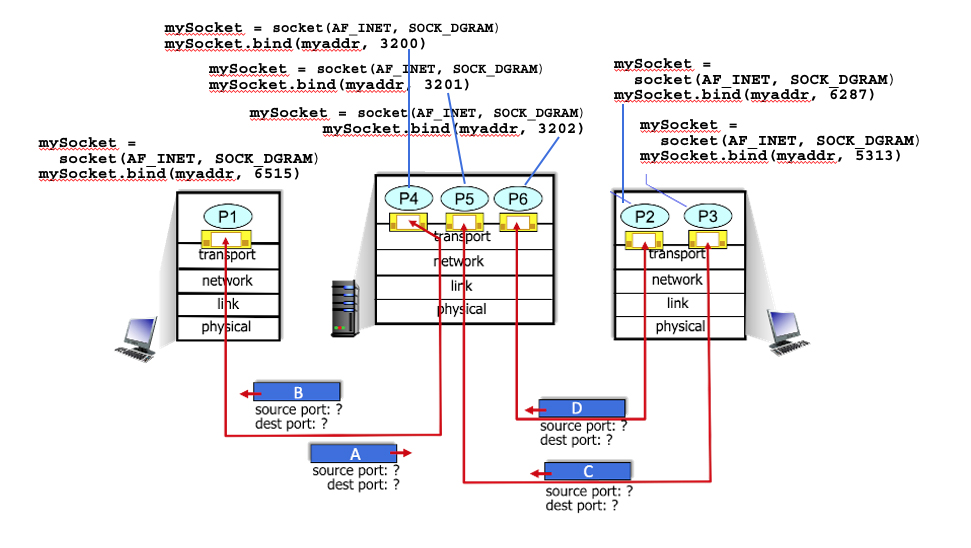
\includegraphics[width=\linewidth]{figs/fig1.jpg}
\end{center}
\item Segmento A porta sorgente \# \answer 6515
\item Segmento B porta sorgente \# \answer 3200
\item Segmento C porta sorgente \# \answer 5313
\item Segmento C porta destinazione \# \answer 3201
\item Segmento D porta sorgente \# \answer 6287
\item Segmento D porta destinazione \# \answer 3202
\end{matching}

\begin{multi}[points=1]{2.2-09. HTTP/2 contro HTTP/1.1: ritardi nel download degli oggetti.}
\textbf{2.2-09. HTTP/2 contro HTTP/1.1: ritardi nel download degli oggetti.}

Si consideri un client e un server, separati da un RTT di 4 unità di tempo. Il client effettua una richiesta per 4 oggetti a $t=0$. $O1$ consiste di 10 frame, $O2$ e $O4$ consistono ciascuno di 1 frame, e $O3$ consiste di 2 frame. Nell'esempio HTTP/2 mostrato nella figura, il server sta trasmettendo frame al client nell'ordine $O1$, $O2$, $O3$, $O4$ (fintanto che ci sono frame del tipo $i$ da trasmettere, e quando non ci sono il server passa semplicemente a un frame dall'oggetto $i+1 mod 4$). Ogni frame impiega 1 unità di tempo per essere trasmesso.

\begin{center}
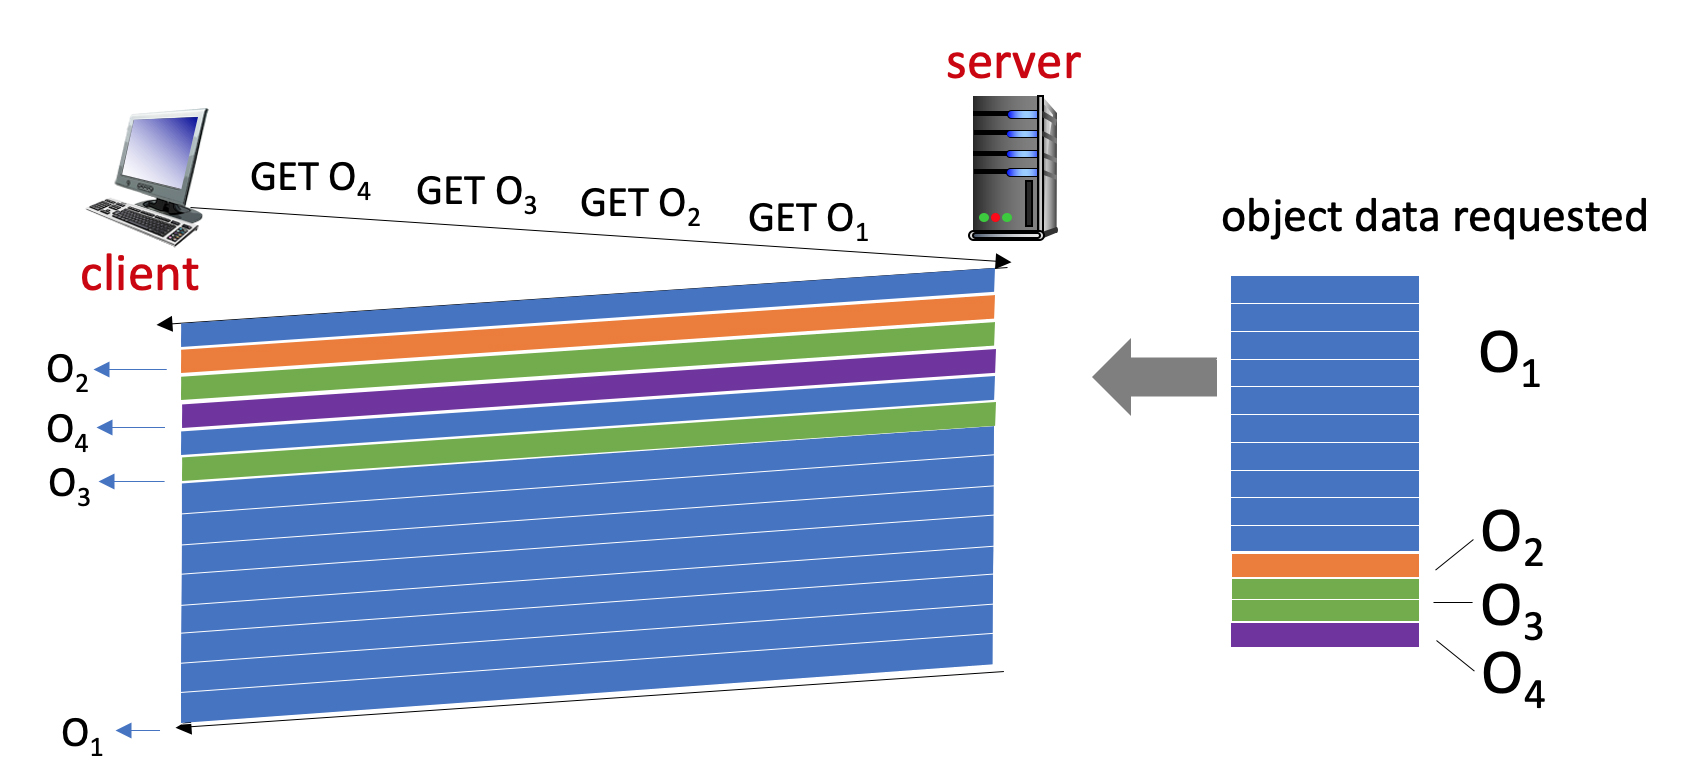
\includegraphics[width=\linewidth]{figs/2.2.9.jpg}
\end{center}

Sotto HTTP 1.1, il server invierebbe $O1$, $O2$, $O3$, $O4$ in quest'ordine in base al principio First-Come-First-Served (FCFS), trasmettendo ogni oggetto nella sua interezza prima di passare a inviare il successivo in quell'ordine. Definiamo ritardo nel download dell'oggetto come il tempo che passa dal momento in cui un oggetto è richiesto (a $t=0$) al momento in cui l'oggetto è ricevuto per intero. Qual è il ritardo medio nel download degli oggetti (la somma dei ritardi nel download dei quattro oggetti divisa per 4) sotto l'ordine di trasmissione dei frame degli oggetti HTTP/2 mostrato nella figura e sotto l'ordine di trasmissione degli oggetti HTTP/1.1 $O1$, $O2$, $O3$, $O4$?
\item* Ritardo medio nel download degli oggetti sotto HTTP/1.1: 16.0, sotto HTTP/2: 10.5
\item Ritardo medio nel download degli oggetti sotto HTTP/1.1: 14.0, sotto HTTP/2: 9.5
\item Ritardo medio nel download degli oggetti sotto HTTP/1.1: 18.0, sotto HTTP/2: 14.0
\item Ritardo medio nel download degli oggetti sotto HTTP/1.1: 12.5, sotto HTTP/2: 10.0
\item Ritardo medio nel download degli oggetti sotto HTTP/1.1: 24.0, sotto HTTP/2: 18.0
\item Ritardo medio nel download degli oggetti sotto HTTP/1.1: 22.0, sotto HTTP/2: 17.5
\end{multi}

\begin{multi}[points=1,shuffle]{2.4-02. DNS: tempo per risolvere la richiesta.}
\textbf{2.4-02. DNS: tempo per risolvere la richiesta.}

Supponi che il server DNS locale metta in cache tutte le informazioni provenienti da tutti i server root, TLD e autoritativi per 20 unità di tempo. Quindi, ad esempio, quando un server root restituisce il nome e l'indirizzo di un server TLD per .com, la cache ricorda che questo è il server TLD da utilizzare per risolvere un nome .com.

Supponi anche che la cache locale sia inizialmente vuota, che vengano sempre utilizzate richieste DNS iterative, che le richieste DNS siano solo per la traduzione del nome in indirizzo IP, che sia necessaria 1 unità di tempo per ogni richiesta o risposta (in una direzione) da server a server o da host a server, e che ci sia solo un server di nome autoritativo (ciascuno) per qualsiasi dominio .edu o .com.
\begin{center}
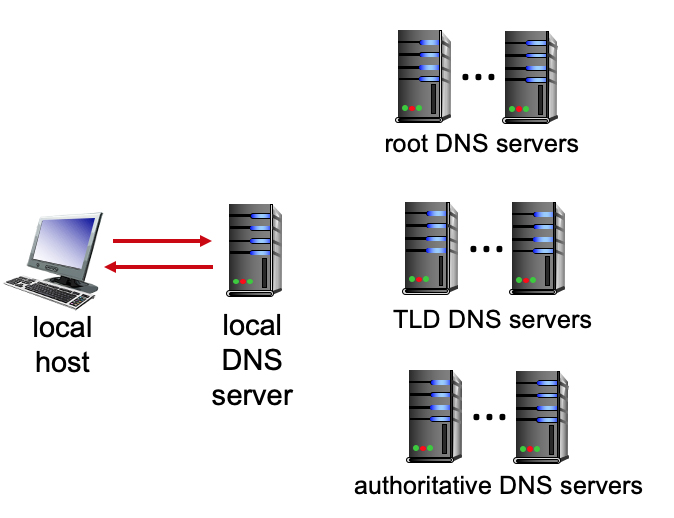
\includegraphics[width=\linewidth]{figs/2.4.4.jpg}
\end{center}

Considera le seguenti richieste DNS, effettuate dall'host locale nei tempi indicati:
\begin{itemize}
	\item $t=0$, l'host locale richiede che il nome gaia.cs.umass.edu sia risolto in un indirizzo IP.
	\item $t=1$, l'host locale richiede che il nome web.cs.umass.edu sia risolto in un indirizzo IP.
\end{itemize}

Quante unità di tempo sono necessarie perché la richiesta DNS effettuata a \textbf{t=1} venga risolta?
\item 2 unità di tempo.
\item 4 unità di tempo.
\item 6 unità di tempo.
\item 8 unità di tempo.
\item* 10 unità di tempo.
\end{multi}

\begin{multi}[points=1,shuffle]{2.6-2 Ritardo nella riproduzione: ritardo minimo nella riproduzione.}
\textbf{2.6-2. Ritardo nella riproduzione: ritardo minimo nella riproduzione.}

Considera lo scenario seguente, in cui un server sta trasmettendo frammenti di video a un client. Il primo frammento è trasmesso dal server a \textbf{t=2}, è ricevuto dal client a \textbf{t=10}, e viene riprodotto dal client a \textbf{t=16}. La ritrasmissione, la ricezione e la riproduzione di 11 frammenti sono mostrate.

In questo esempio, il ritardo nella riproduzione è 6, e nessun frammento perde la propria scadenza di riproduzione.
\begin{center}
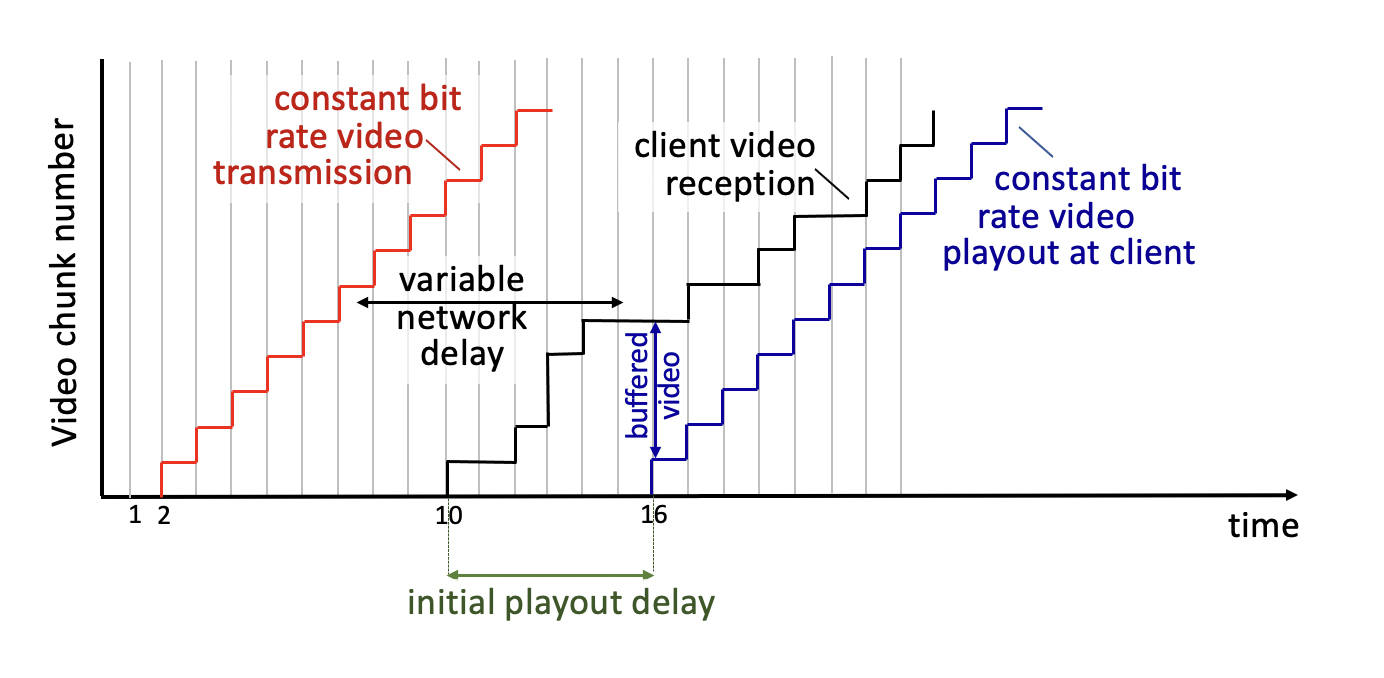
\includegraphics[width=\linewidth]{figs/playout_delay.jpg}
\end{center}

Qual è il \textbf{minimo} ritardo iniziale di riproduzione tale per cui la riproduzione (periodica) dei frammenti è temporizzata in modo che nessun frammento perda la propria scadenza di riproduzione? Puoi assumere che se un frammento arriva (scala nera) nello stesso momento in cui è programmato per la riproduzione (scala blu), allora il frammento viene riprodotto con successo senza essere perso.
\item 1
\item 2
\item 3
\item* 4
\item 5
\item 6
\item Non è possibile.
\end{multi}

\begin{multi}[points=1,shuffle]{3.5-2a. Numeri di sequenza e di ACK di TCP.}
\textbf{3.5-2a. Numeri di sequenza e di ACK di TCP.}

Considera la figura seguente, dove un mittente TCP invia 8 segmenti TCP a \emph{t = 1, 2, 3, 4, 5, 6, 7, 8.} Supponiamo che il valore iniziale del numero di sequenza sia 0 e che ogni segmento inviato al ricevente contenga 100 byte. Il ritardo tra il mittente e il ricevente è di 5 unità di tempo, quindi il primo segmento arriva al ricevente a t = 6. Gli ACK inviati dal ricevente a \emph{t = 6, 7, 8, 10, 11, 12} sono mostrati. I segmenti TCP (se presenti) inviati dal mittente a \emph{t = 11, 13, 15, 16, 17, 18} \emph{non} sono mostrati. Il segmento inviato a \emph{t=4} viene perso, così come il segmento ACK inviato a \emph{t=7}.
\begin{center}
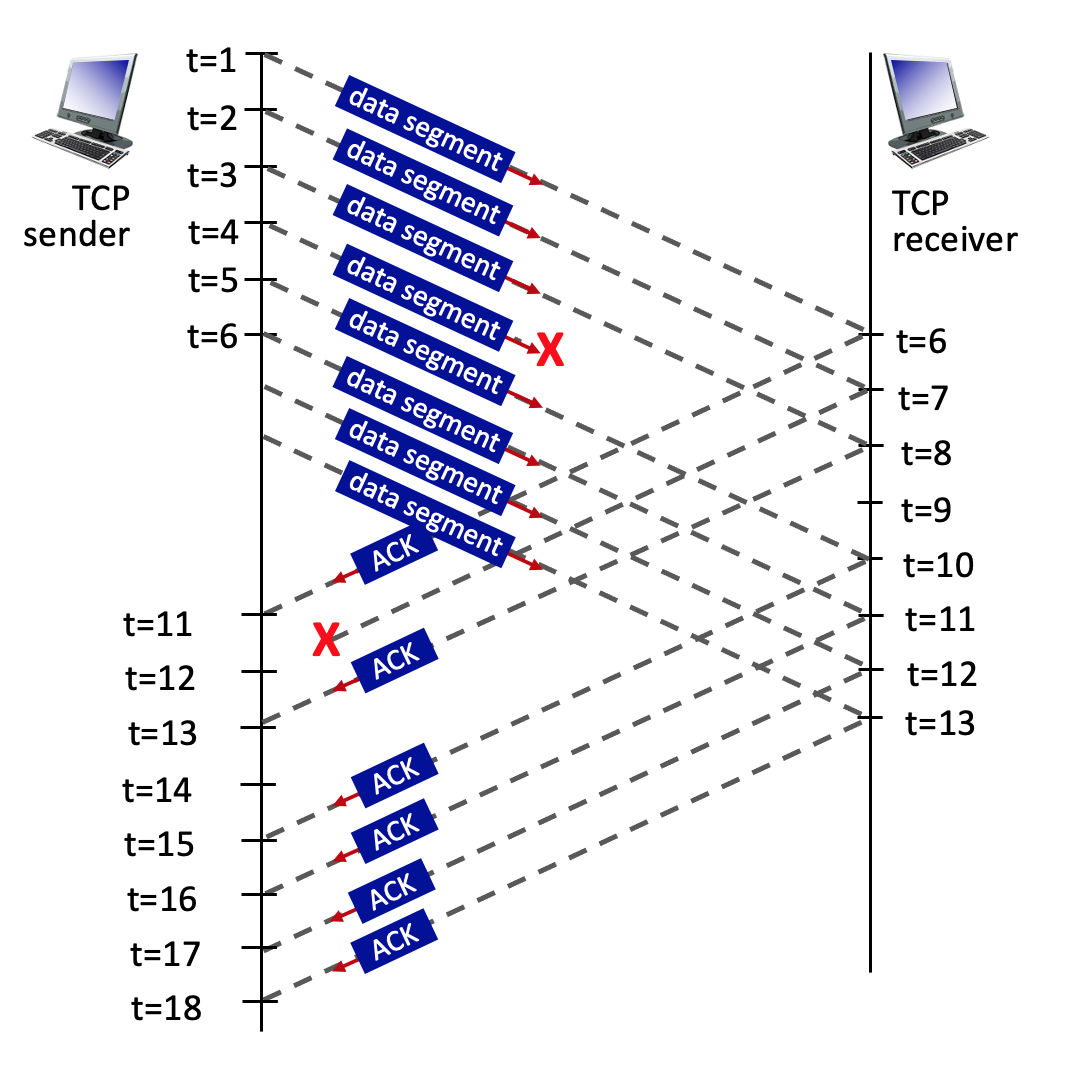
\includegraphics[width=\linewidth]{figs/tcp_seq_ack_1.jpg}
\end{center}

 Qual è il numero di sequenza del segmento inviato a \emph{t=2}?
\item 200
\item* 100
\item 1
\item 2
\end{multi}

\begin{multi}[points=1,shuffle]{3.5-2b. Numeri di sequenza e di ACK TCP (b).}
\textbf{3.5-2b. Numeri di sequenza e di ACK TCP (b). }

Considera di nuovo la figura sottostante (come nella domanda 3.5-2a) dove un mittente TCP invia 8 segmenti TCP a \emph{t = 1, 2, 3, 4, 5, 6, 7, 8} e il segmento inviato a \emph{t=4} viene perso, così come il segmento di ACK inviato a \emph{t=7}. Qual è il valore di ACK nella risposta dal ricevitore al mittente inviata a \emph{t=6}?
\begin{center}
	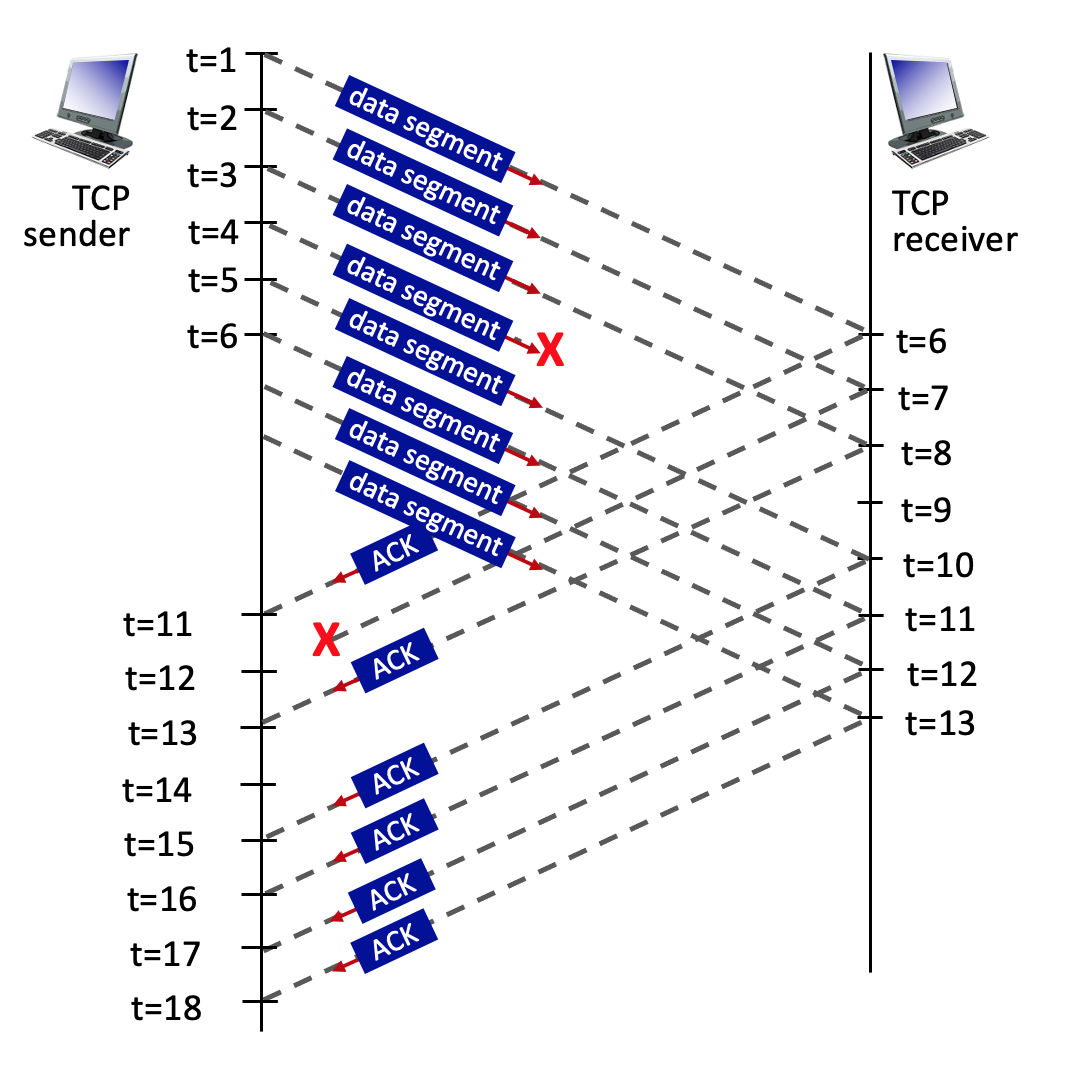
\includegraphics[width=\linewidth]{figs/tcp_seq_ack_1.jpg}
\end{center}
\item 200
\item* 100
\item 1
\item 2
\item 0
\item Nessuna di queste altre risposte.
\end{multi}

\begin{multi}[points=1,shuffle]{3.5-2c. Sequenza e numeri di ACK TCP (c).}
\textbf{3.5-2c. Sequenza e numeri di ACK TCP (c).}

Prendi nuovamente in considerazione la figura sottostante (come nella domanda 3.5-2a) dove un mittente TCP invia 8 segmenti TCP a \emph{t = 1, 2, 3, 4, 5, 6, 7, 8} e il segmento inviato a \emph{t=4} viene perso, così come il segmento di ACK inviato a \emph{t=7}. Qual è il valore di ACK trasportato nell'ACK da ricevitore a mittente inviato a \emph{t=8}?
\begin{center}
	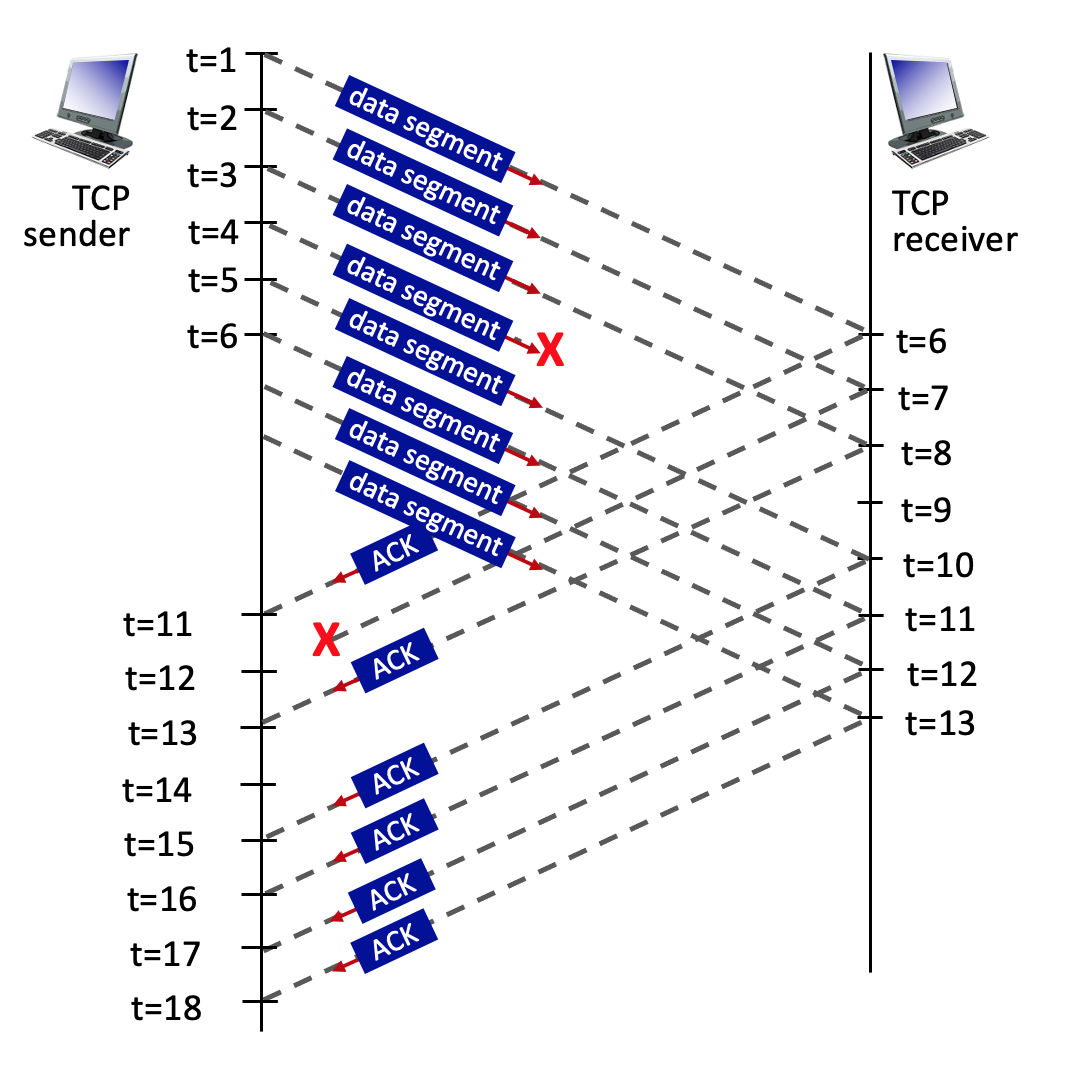
\includegraphics[width=\linewidth]{figs/tcp_seq_ack_1.jpg}
\end{center}
\item 200
\item 100
\item* 300
\item 400
\item 3
\item Nessuna di queste altre risposte.
\end{multi}

\begin{multi}[points=1,shuffle]{3.5-2d. Numeri di sequenza e di ACK in TCP (d).}
\textbf{3.5-2d. Numeri di sequenza e di ACK in TCP (d).}

Considera di nuovo la figura qui sotto (come nella domanda 3.5-2a) dove un mittente TCP invia 8 segmenti TCP a \emph{t = 1, 2, 3, 4, 5, 6, 7, 8} e il segmento inviato a \emph{t=4} viene perso, così come il segmento ACK inviato a \emph{t=7}. Qual è il valore di ACK trasmesso nell'ACK da ricevitore a mittente inviato a \emph{t=10}?
\begin{center}
	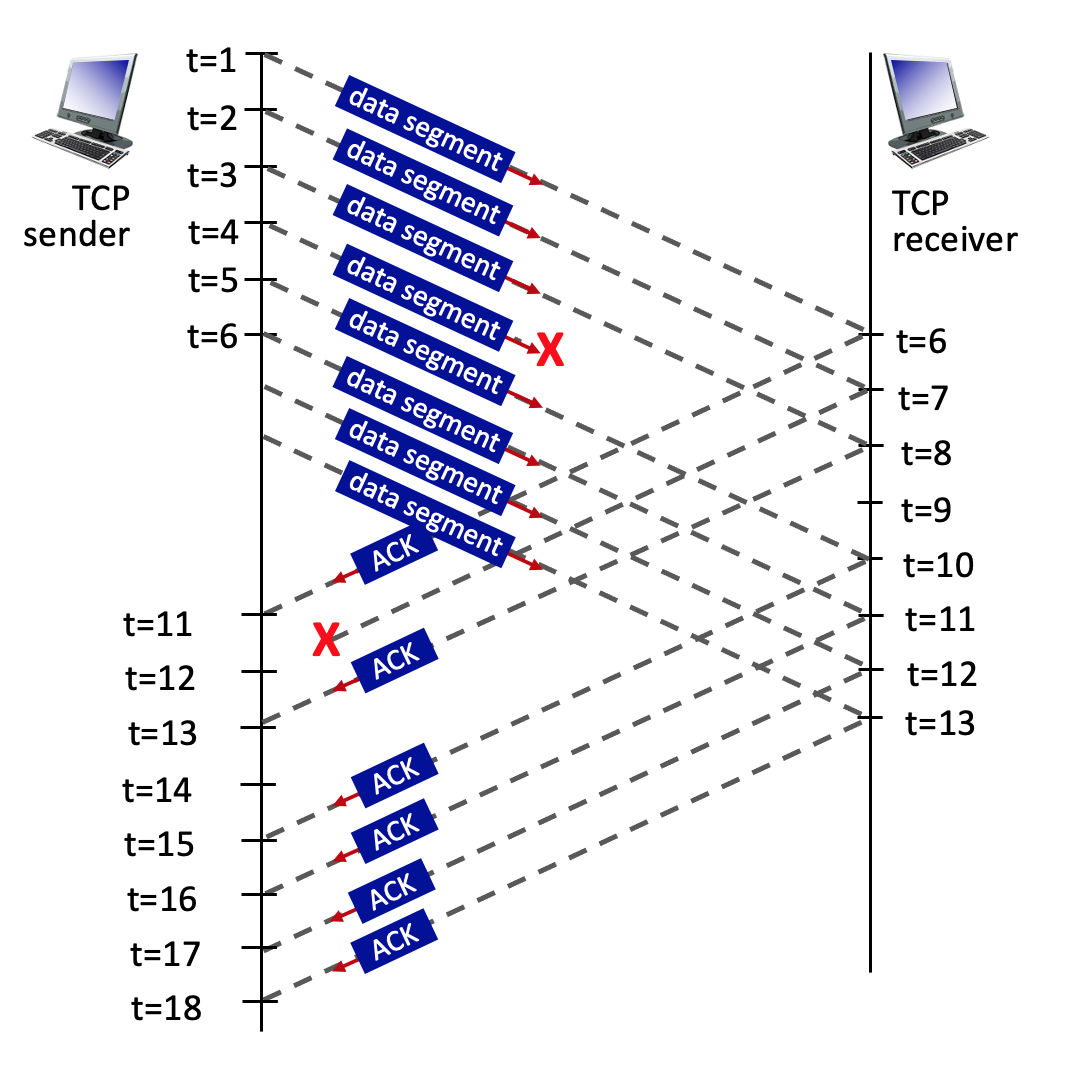
\includegraphics[width=\linewidth]{figs/tcp_seq_ack_1.jpg}
\end{center}
\item 200
\item 100
\item* 300
\item 400
\item 3
\item Nessuna di queste altre risposte.
\end{multi}

\begin{multi}[points=1,shuffle]{3.7-1a. Esempio di controllo della congestione TCP (a).}
\textbf{3.7-1a. Esempio di controllo della congestione TCP (a).}

Considera la figura sottostante, dove un mittente TCP invia 8 segmenti TCP ai tempi \emph{t = 1, 2, 3, 4, 5, 6, 7, 8.} Supponi che il valore iniziale del numero di sequenza sia 0 e che ogni segmento inviato al ricevente contenga 100 byte. Il ritardo tra il mittente e il ricevente è di 5 unità di tempo, quindi il primo segmento arriva al ricevente a \textbf{t=6}. Gli ACK inviati dal ricevente ai tempi \emph{t = 6, 7, 8, 10, 11, 12} sono mostrati. I segmenti TCP (se presenti) inviati dal mittente ai tempi \textbf{t = 11, 13, 15, 16, 17, 18} \emph{non} sono mostrati. Il segmento inviato a \textbf{t=4} è perso, così come il segmento ACK inviato a \textbf{t=7}.

\begin{center}
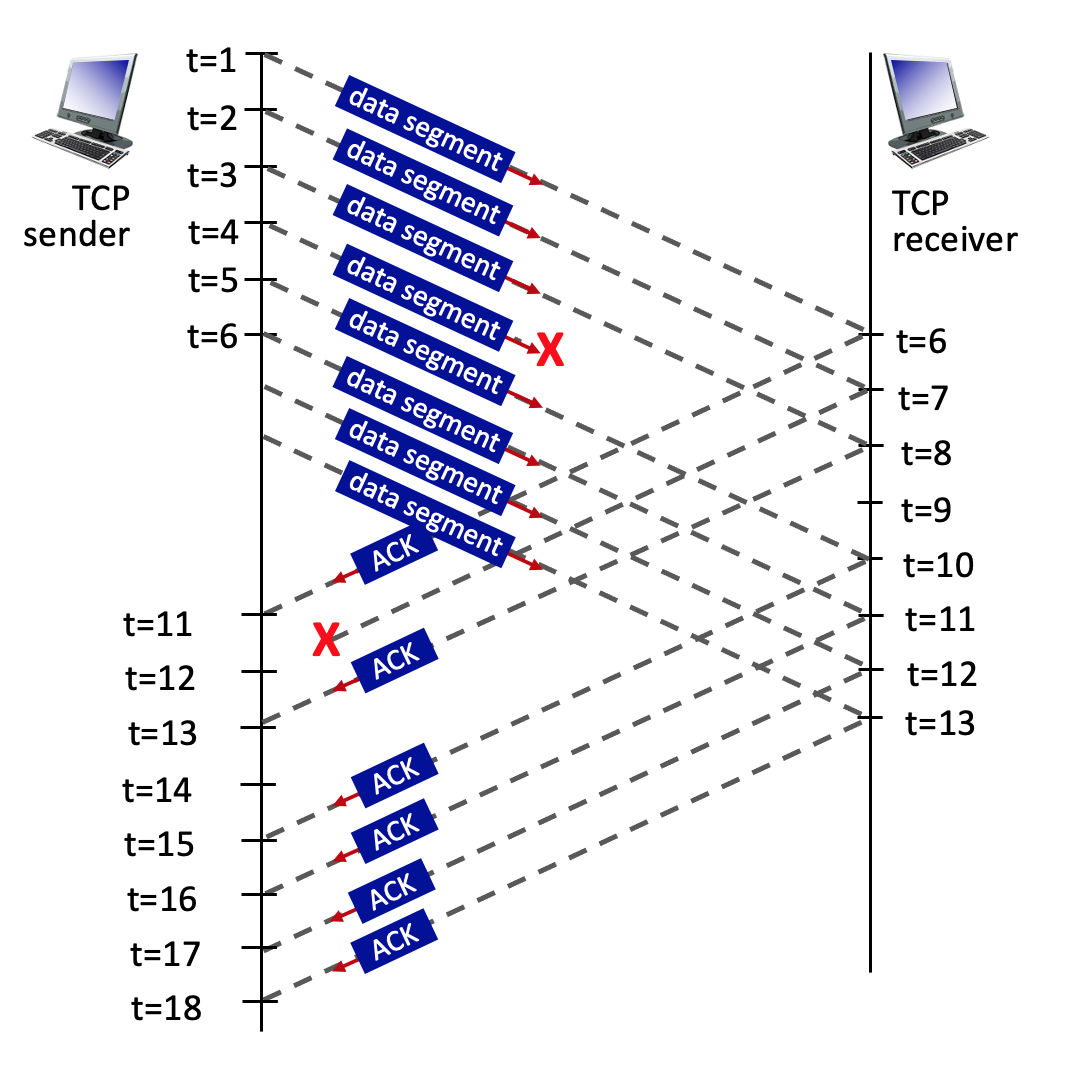
\includegraphics[width=\linewidth]{figs/tcp_seq_ack_1.jpg}
\end{center}

Qual è l'azione del mittente a \textbf{t = 11} alla ricezione dell'ACK?
\item Aumenta la dimensione della finestra di congestione, sposta in avanti la base della finestra di 2 e invia nuovi segmenti, se disponibili e come consentito dalla finestra di congestione.
\item* Aumenta la dimensione della finestra di congestione, sposta in avanti la base della finestra di 1 e invia nuovi segmenti, se disponibili e come consentito dalla finestra di congestione.
\item Mantieni la dimensione della finestra di congestione invariata ma invia nuovi segmenti, se disponibili e come consentito dalla finestra di congestione.
\item Non fare nulla.
\item Invia un ACK per l'ACK.
\end{multi}

\begin{multi}[points=1,shuffle]{3.7-1b. Esempio di controllo della congestione TCP (b).}
\textbf{3.7-1b. Esempio di controllo della congestione TCP (b).}

Considera nuovamente la figura sottostante (come nella domanda 3.7-1a), dove un mittente TCP invia 8 segmenti TCP a \emph{t = 1, 2, 3, 4, 5, 6, 7, 8} e il segmento inviato a \textbf{t=4} si perde, così come il segmento ACK inviato a \textbf{t=7}.

\begin{center}
	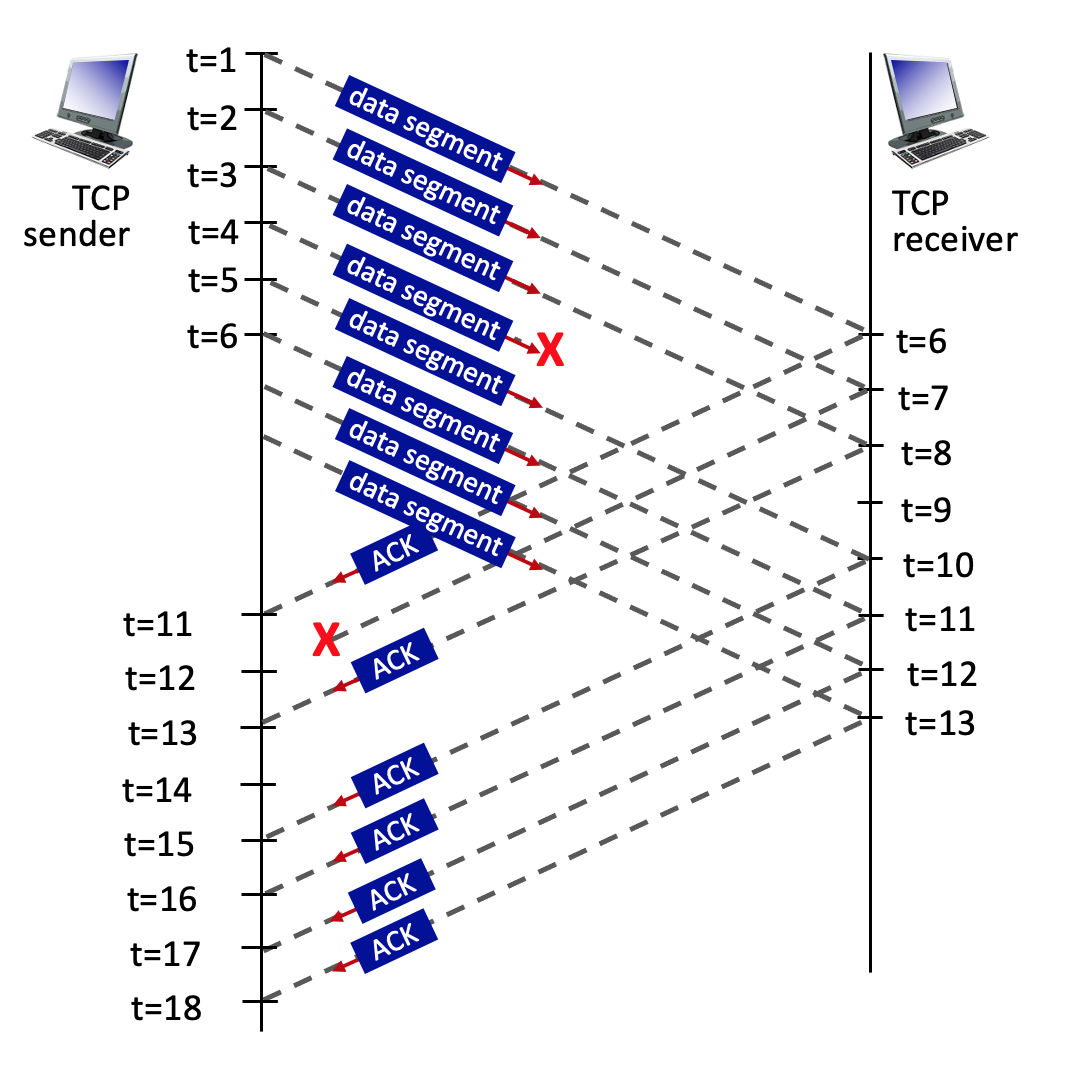
\includegraphics[width=\linewidth]{figs/tcp_seq_ack_1.jpg}
\end{center}

Qual è l'azione del mittente a \textbf{t=13} al ricevimento dell'ACK?
\item* Aumenta la dimensione della finestra di congestione, sposta in avanti la base della finestra di 2 e invia nuovi segmenti, se disponibili e come consentito dalla finestra di congestione.
\item Aumenta la dimensione della finestra di congestione, sposta in avanti la base della finestra di 1 e invia nuovi segmenti, se disponibili e come consentito dalla finestra di congestione.
\item Mantieni la dimensione della finestra di congestione invariata. Incrementa il conteggio degli ACK duplicati di 1.
\item Non fa nulla.
\item Invia un ACK per l'ACK.
\end{multi}

\begin{multi}[points=1,shuffle]{3.7-1c. Esempio di controllo della congestione TCP (c).}
\textbf{3.7-1c. Esempio di controllo della congestione TCP (c).}

Considera ancora la figura sottostante (come nella domanda 3.7-1a), dove un mittente TCP invia 8 segmenti TCP a \emph{t = 1, 2, 3, 4, 5, 6, 7, 8} e il segmento inviato a \textbf{t=4} è perso, così come il segmento ACK inviato a \textbf{t=7}.

\begin{center}
	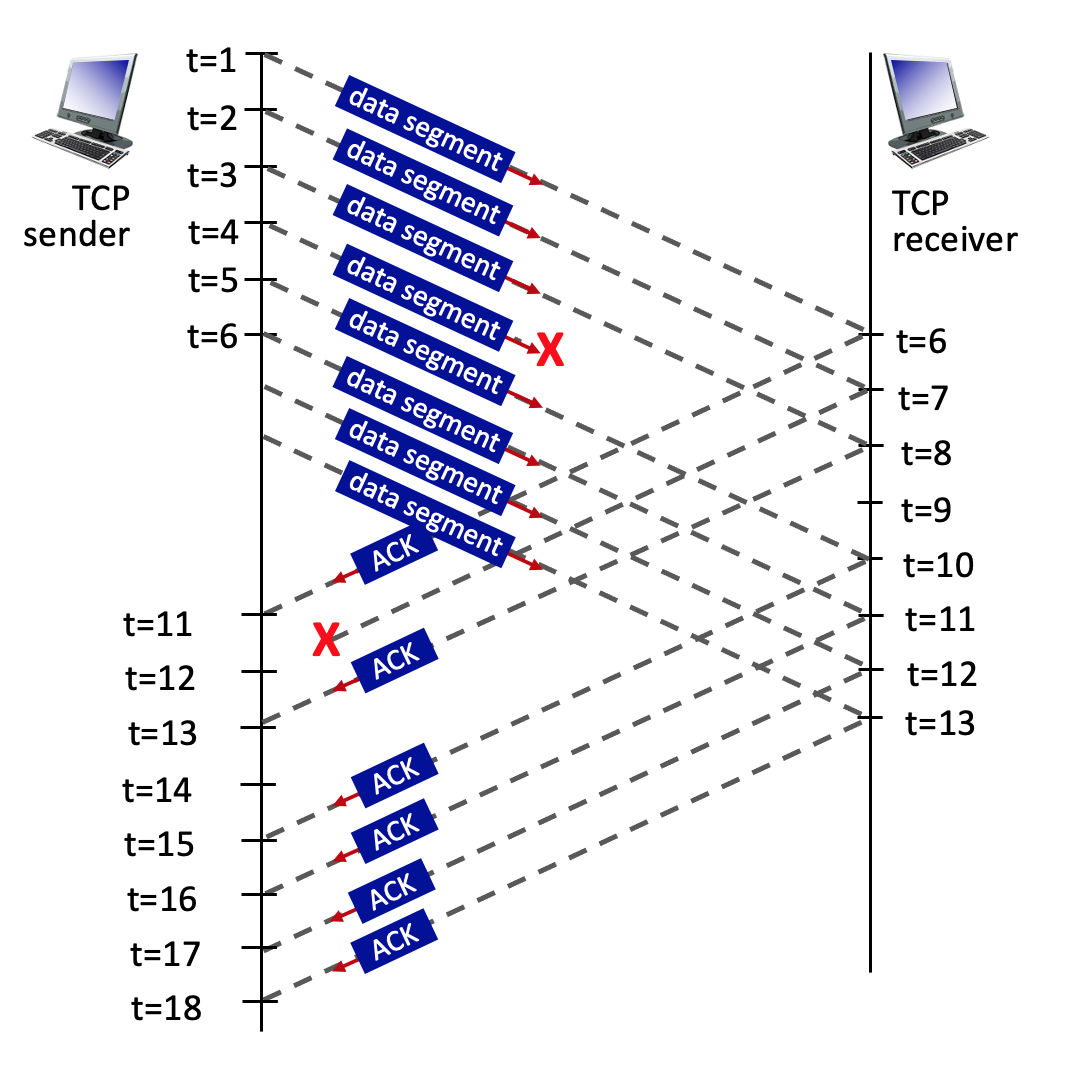
\includegraphics[width=\linewidth]{figs/tcp_seq_ack_1.jpg}
\end{center}

Cosa fa il mittente a \textbf{t=16}? Puoi assumere per questa domanda che non si siano verificati timeout.
\item Imposta il valore della sua finestra cwnd a 1 e ritrasmette il segmento con numero di sequenza 300.
\item Taglia a metà il valore della sua cwnd e ritrasmette il segmento con numero di sequenza 300.
\item Informa lo strato superiore che la connessione è terminata e chiude il socket.
\item* Non fa nulla se non incrementare il numero di ACK duplicati di 1.
\end{multi}

\begin{multi}[points=1,shuffle]{3.7-1d. Esempio di controllo della congestione TCP (d).}
\textbf{3.7-1d Esempio di controllo della congestione TCP (d).}

Considera nuovamente la figura sottostante (come nella domanda 3.7-1a), dove un mittente TCP invia 8 segmenti TCP ai tempi \emph{t = 1, 2, 3, 4, 5, 6, 7, 8} e il segmento inviato a \textbf{t=4} viene perso, così come il segmento ACK inviato a \textbf{t=7}.

\begin{center}
	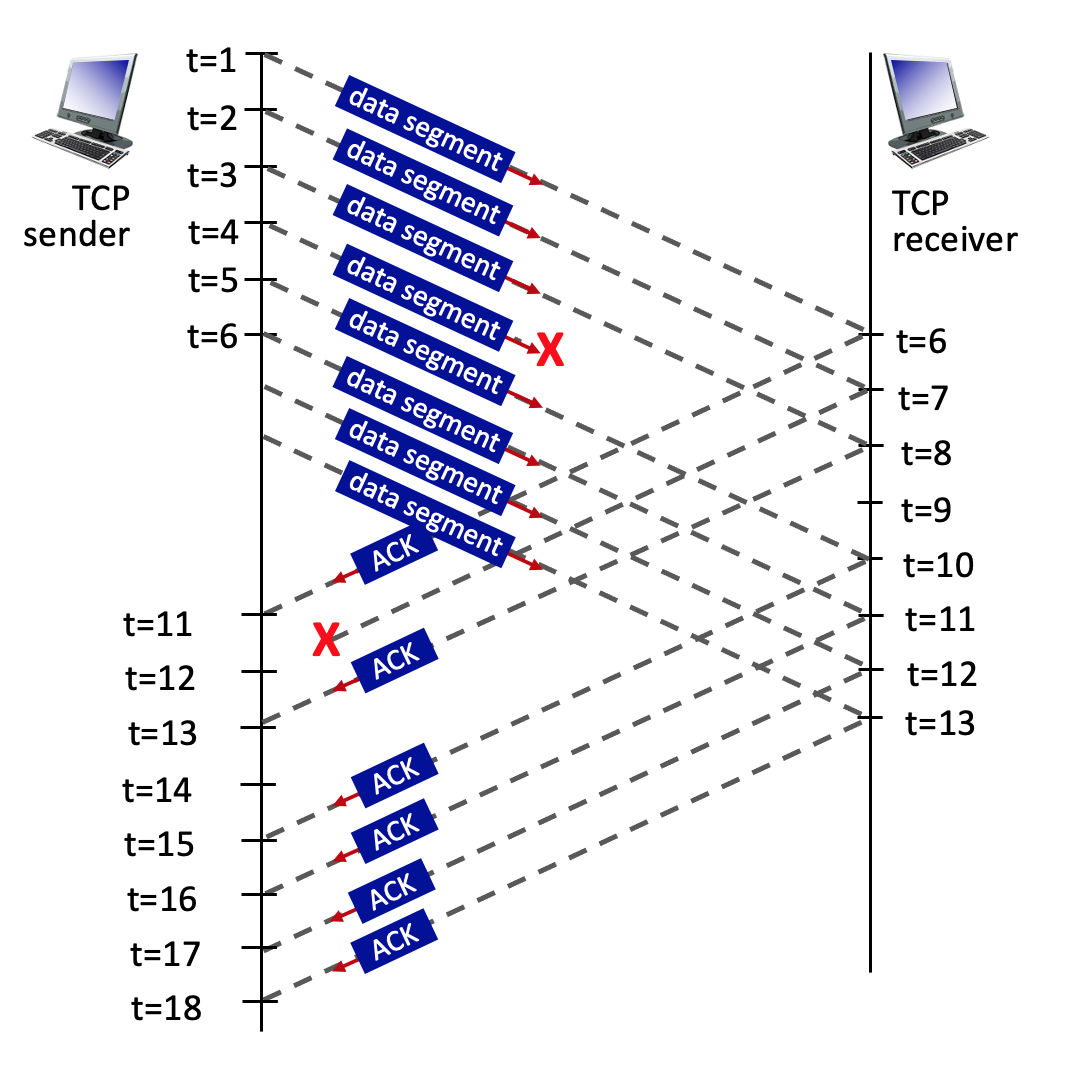
\includegraphics[width=\linewidth]{figs/tcp_seq_ack_1.jpg}
\end{center}

Cosa fa il mittente a \textbf{t=17}? Puoi assumere per questa domanda che non si siano verificati timeout.
\item Imposta il valore della sua finestra cwnd a 1 e ritrasmette il segmento con numero di sequenza 300.
\item* Taglia a metà il valore della sua cwnd e ritrasmette il segmento con numero di sequenza 300.
\item Informa lo strato superiore che la connessione è terminata e chiude il socket.
\item Non fa nulla se non incrementare il numero di ACK duplicati di 1.
\end{multi}

\begin{multi}[points=1,shuffle]{3.7-1e. Esempio di controllo della congestione TCP (e).}
\textbf{3.7-1e. Esempio di controllo della congestione TCP (e).}

Considera di nuovo la figura sottostante (come nella domanda 3.7-1a), dove un mittente TCP invia 8 segmenti TCP a \emph{t = 1, 2, 3, 4, 5, 6, 7, 8} e il segmento inviato a \textbf{t=4} viene perso, come anche il segmento ACK inviato a \textbf{t=7}.

\begin{center}
	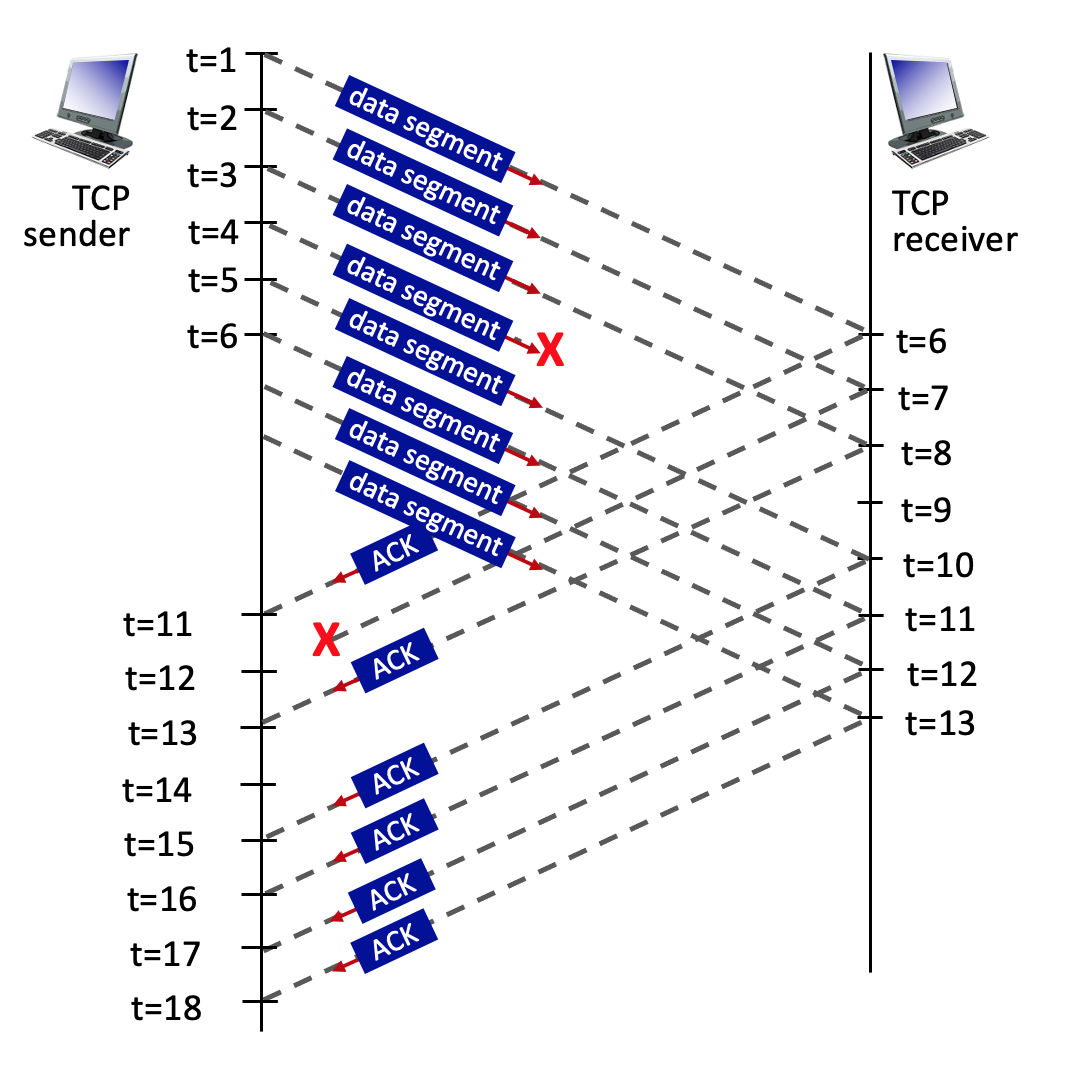
\includegraphics[width=\linewidth]{figs/tcp_seq_ack_1.jpg}
\end{center}

Supponi che il prossimo evento dopo \textbf{t=17} sia un evento di timeout. Cosa fa il mittente?
\item* Imposta il valore della sua finestra cwnd a 1 e ritrasmette il segmento con numero di sequenza 300.
\item Imposta il valore della sua finestra cwnd a 1, a, e ritrasmette il segmento con numero di sequenza 100.
\item Informa il livello superiore che la connessione è terminata e chiude il socket.
\item Non fa nulla.
\item Taglia a metà il valore della sua finestra cwnd e ritrasmette il segmento con numero di sequenza 300.
\end{multi}

\begin{multi}[points=1,shuffle,multiple]{3.7-2a. Fasi del controllo della congestione TCP (a).}
\textbf{3.7-2a Fasi del controllo della congestione TCP (a).} 

Considerare la figura sottostante, che traccia l'evoluzione della finestra di congestione di TCP all'inizio di ogni unità di tempo (dove l'unità di tempo è pari al RTT). Nel modello astratto per questo problema, TCP invia una ``serie'' di pacchetti di dimensione cwnd all'inizio di ogni unità di tempo. Il risultato dell'invio di quella serie di pacchetti è che o (i) tutti i pacchetti sono ACKed alla fine dell'unità di tempo, (ii) si verifica un timeout per il primo pacchetto, oppure (iii) si verifica un triplice duplicate ACK per il primo pacchetto.

Durante quali dei seguenti intervalli di tempo TCP sta eseguendo lo slow start?
\begin{center}
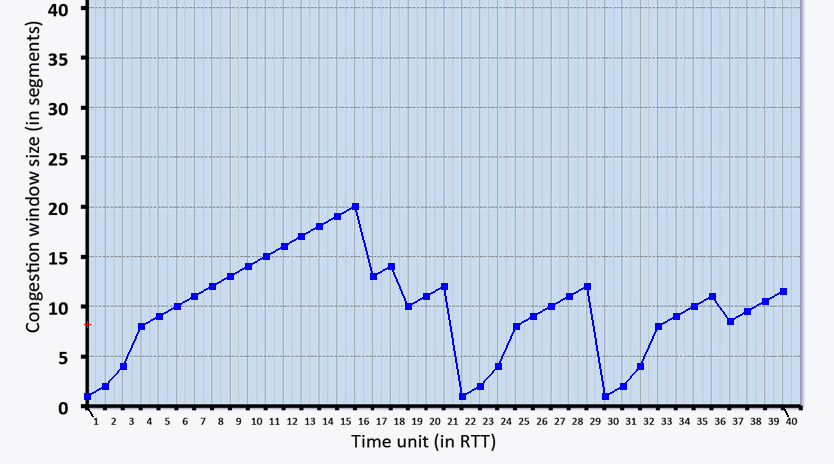
\includegraphics[width=\linewidth]{figs/tcp_cc_evolution.jpg}
\end{center}

\item[fraction=50] $[1,3]$
\item $[4,15]$
\item 16
\item 17
\item 18
\item $[19,20]$
\item 21
\item[fraction=50] $[22,24]$
\end{multi}

\begin{multi}[points=1,shuffle,multiple]{3.7-2b. Fasi del controllo della congestione di TCP (b).}
\textbf{3.7-2b Fasi del controllo della congestione di TCP (b).}

Considera nuovamente la figura sottostante (come nella domanda 3.7-2a) che mostra l'evoluzione delle dimensioni della finestra di congestione di TCP. In questa figura, durante quali dei seguenti intervalli di tempo TCP è in congestion avoidance?

\begin{center}
	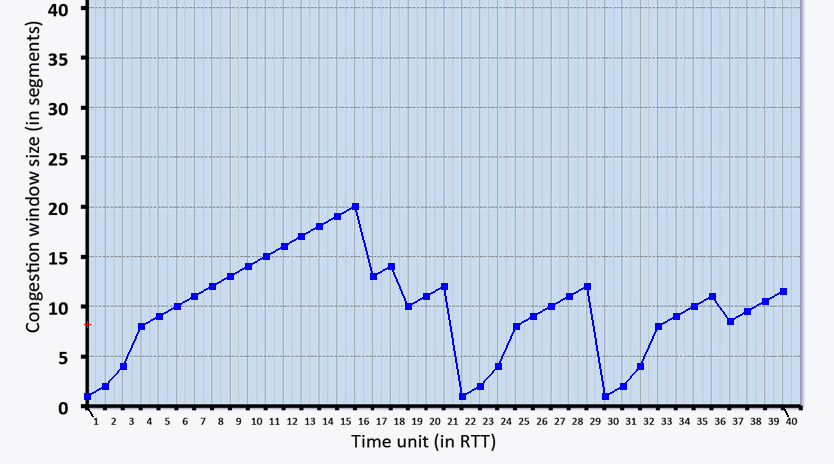
\includegraphics[width=\linewidth]{figs/tcp_cc_evolution.jpg}
\end{center}
\item $[1,3]$
\item[fraction=33.33333] $[4,15]$
\item 16
\item[fraction=33.33333] 17
\item 18
\item[fraction=33.33333] $[19,20]$
\item 21
\item $[22,24]$
\end{multi}

\begin{multi}[points=1,shuffle,multiple]{3.7-2c Fasi del controllo di congestione TCP (c).}
\textbf{3.7-2c Fasi del controllo di congestione TCP (c).} 

Considera nuovamente la figura sottostante (come nella domanda 3.7-2a) che mostra l'evoluzione della dimensione della finestra di congestione di TCP. In questa figura, al termine di quali unità di tempo TCP rileva un triple-duplicate-ACK?

\begin{center}
	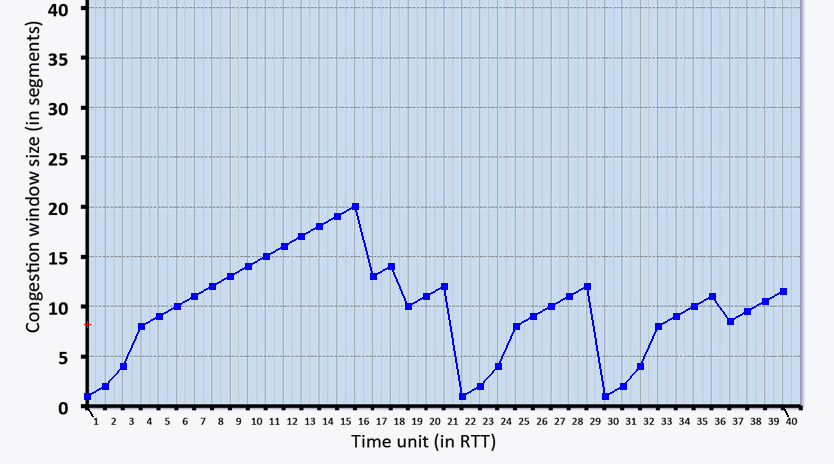
\includegraphics[width=\linewidth]{figs/tcp_cc_evolution.jpg}
\end{center}
\item $[1,3]$
\item $[4,15]$
\item[fraction=50] 16
\item 17
\item[fraction=50] 18
\item $[19,20]$
\item 21
\item $[22,24]$
\end{multi}

\begin{multi}[points=1,shuffle]{3.7-2d. Fasi del controllo della congestione TCP (d).}
\textbf{3.7-2d. Fasi del controllo della congestione TCP (d).}

Considera nuovamente la figura sopra (domanda 3.7-2a) che mostra l'evoluzione della dimensione della finestra di congestione di TCP. In questa figura, alla fine di quale/i unità/i di tempo TCP rileva una perdita tramite timeout?

\begin{center}
	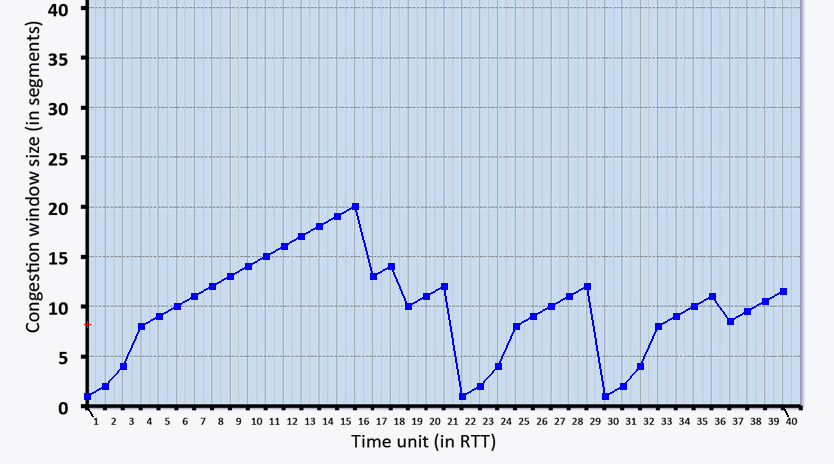
\includegraphics[width=\linewidth]{figs/tcp_cc_evolution.jpg}
\end{center}
\item $[1,3]$
\item $[4,15]$
\item 16
\item 17
\item 18
\item $[19,20]$
\item* 21
\item $[22,24]$
\end{multi}

\begin{shortanswer}[points=1,shuffle]{3.5-1a. Stima del RTT e valore di timeout TCP.}
\textbf{3.5-1a. Stima del RTT e valore di timeout TCP}.

Supponiamo che i valori correnti stimati di TCP per il tempo di andata e ritorno (\textbf{estimatedRTT}) e la deviazione nel RTT (\textbf{DevRTT}) siano rispettivamente 300 msec e 13 msec. Supponiamo che i prossimi due RTT misurati siano rispettivamente 330 msec e 240 msec.

Vogliamo calcolare la stima del RTT di TCP e il valore dell'intervallo di timeout di TCP. Nota che dato un nuovo RTT misurato, si dovrebbe prima calcolare \textbf{devRTT}, poi \textbf{estimatedRTT}, e infine (per ultimo) l'intervallo di timeout.

Usa i valori di $\alpha$ = 0.125, $\beta$ = 0.25. Seguendo il nuovo RTT misurato di 330 msec, qual è il nuovo valore per \textbf{devRTT} in msec? [Nota: arrotonda la tua risposta al msec più vicino -- inserisci un valore intero, non includere nessun decimale o zeri iniziali]
\item* 17
\end{shortanswer}

\end{quiz}
\end{document}

